%  LaTeX support: latex@mdpi.com
%  For support, please attach all files needed for compiling as well as the log file, and specify your operating system, LaTeX version, and LaTeX editor.

%=================================================================
% pandoc conditionals added to preserve backwards compatibility with previous versions of rticles

\documentclass[notspecified,article,submit,moreauthors,pdftex]{Definitions/mdpi}


%% Some pieces required from the pandoc template
\setlist[itemize]{leftmargin=*,labelsep=5.8mm}
\setlist[enumerate]{leftmargin=*,labelsep=4.9mm}


%--------------------
% Class Options:
%--------------------

%---------
% article
%---------
% The default type of manuscript is "article", but can be replaced by:
% abstract, addendum, article, book, bookreview, briefreport, casereport, comment, commentary, communication, conferenceproceedings, correction, conferencereport, entry, expressionofconcern, extendedabstract, datadescriptor, editorial, essay, erratum, hypothesis, interestingimage, obituary, opinion, projectreport, reply, retraction, review, perspective, protocol, shortnote, studyprotocol, systematicreview, supfile, technicalnote, viewpoint, guidelines, registeredreport, tutorial
% supfile = supplementary materials

%----------
% submit
%----------
% The class option "submit" will be changed to "accept" by the Editorial Office when the paper is accepted. This will only make changes to the frontpage (e.g., the logo of the journal will get visible), the headings, and the copyright information. Also, line numbering will be removed. Journal info and pagination for accepted papers will also be assigned by the Editorial Office.

%------------------
% moreauthors
%------------------
% If there is only one author the class option oneauthor should be used. Otherwise use the class option moreauthors.

%---------
% pdftex
%---------
% The option pdftex is for use with pdfLaTeX. Remove "pdftex" for (1) compiling with LaTeX & dvi2pdf (if eps figures are used) or for (2) compiling with XeLaTeX.

%=================================================================
% MDPI internal commands - do not modify
\firstpage{1}
\makeatletter
\setcounter{page}{\@firstpage}
\makeatother
\pubvolume{1}
\issuenum{1}
\articlenumber{0}
\pubyear{2023}
\copyrightyear{2023}
%\externaleditor{Academic Editor: Firstname Lastname}
\datereceived{ }
\daterevised{ } % Comment out if no revised date
\dateaccepted{ }
\datepublished{ }
%\datecorrected{} % For corrected papers: "Corrected: XXX" date in the original paper.
%\dateretracted{} % For corrected papers: "Retracted: XXX" date in the original paper.
\hreflink{https://doi.org/} % If needed use \linebreak
%\doinum{}
%\pdfoutput=1 % Uncommented for upload to arXiv.org

%=================================================================
% Add packages and commands here. The following packages are loaded in our class file: fontenc, inputenc, calc, indentfirst, fancyhdr, graphicx, epstopdf, lastpage, ifthen, float, amsmath, amssymb, lineno, setspace, enumitem, mathpazo, booktabs, titlesec, etoolbox, tabto, xcolor, colortbl, soul, multirow, microtype, tikz, totcount, changepage, attrib, upgreek, array, tabularx, pbox, ragged2e, tocloft, marginnote, marginfix, enotez, amsthm, natbib, hyperref, cleveref, scrextend, url, geometry, newfloat, caption, draftwatermark, seqsplit
% cleveref: load \crefname definitions after \begin{document}

%=================================================================
% Please use the following mathematics environments: Theorem, Lemma, Corollary, Proposition, Characterization, Property, Problem, Example, ExamplesandDefinitions, Hypothesis, Remark, Definition, Notation, Assumption
%% For proofs, please use the proof environment (the amsthm package is loaded by the MDPI class).

%=================================================================
% Full title of the paper (Capitalized)
\Title{Análisis del mercado laboral en España}

% MDPI internal command: Title for citation in the left column
\TitleCitation{Análisis del mercado laboral en España}

% Author Orchid ID: enter ID or remove command
%\newcommand{\orcidauthorA}{0000-0000-0000-000X} % Add \orcidA{} behind the author's name
%\newcommand{\orcidauthorB}{0000-0000-0000-000X} % Add \orcidB{} behind the author's name


% Authors, for the paper (add full first names)
\Author{Catret Ruber, Pablo$^{1}$, Palazón Caballero, José
Miguel$^{1,*}$, Rosique Martínez, Marcos$^{1}$}


%\longauthorlist{yes}


% MDPI internal command: Authors, for metadata in PDF
\AuthorNames{Catret Ruber, Pablo, Palazón Caballero, José
Miguel, Rosique Martínez, Marcos}

% MDPI internal command: Authors, for citation in the left column
%\AuthorCitation{Lastname, F.; Lastname, F.; Lastname, F.}
% If this is a Chicago style journal: Lastname, Firstname, Firstname Lastname, and Firstname Lastname.
\AuthorCitation{Catret Ruber, P.; Palazón Caballero, J.M.; Rosique
Martínez, M.}

% Affiliations / Addresses (Add [1] after \address if there is only one affiliation.)
\address{%
$^{1}$ \quad Universitat de València - Escola Tècnica Superior
d'Enginyeria (ETSE) Avinguda de l'Universitat, 46100 Burjassot,
Valencia; \\
}

% Contact information of the corresponding author
\corres{Correspondence: \href{mailto:jomipaca@alumni.uv.es}{\nolinkurl{jomipaca@alumni.uv.es}}.}

% Current address and/or shared authorship








% The commands \thirdnote{} till \eighthnote{} are available for further notes

% Simple summary
\simplesumm{A Simple summary goes here.}

%\conference{} % An extended version of a conference paper

% Abstract (Do not insert blank lines, i.e. \\)
\abstract{A single paragraph of about 200 words maximum. For research
articles, abstracts should give a pertinent overview of the work. We
strongly encourage authors to use the following style of structured
abstracts, but without headings: 1) Background: Place the question
addressed in a broad context and highlight the purpose of the study; 2)
Methods: Describe briefly the main methods or treatments applied; 3)
Results: Summarize the article's main findings; and 4) Conclusion:
Indicate the main conclusions or interpretations. The abstract should be
an objective representation of the article, it must not contain results
which are not presented and substantiated in the main text and should
not exaggerate the main conclusions.}


% Keywords
\keyword{keyword 1; keyword 2; keyword 3 (list three to ten pertinent
keywords specific to the article, yet reasonably common within the
subject discipline.).}

% The fields PACS, MSC, and JEL may be left empty or commented out if not applicable
%\PACS{J0101}
%\MSC{}
%\JEL{}

%%%%%%%%%%%%%%%%%%%%%%%%%%%%%%%%%%%%%%%%%%
% Only for the journal Diversity
%\LSID{\url{http://}}

%%%%%%%%%%%%%%%%%%%%%%%%%%%%%%%%%%%%%%%%%%
% Only for the journal Applied Sciences

%%%%%%%%%%%%%%%%%%%%%%%%%%%%%%%%%%%%%%%%%%

%%%%%%%%%%%%%%%%%%%%%%%%%%%%%%%%%%%%%%%%%%
% Only for the journal Data



%%%%%%%%%%%%%%%%%%%%%%%%%%%%%%%%%%%%%%%%%%
% Only for the journal Toxins


%%%%%%%%%%%%%%%%%%%%%%%%%%%%%%%%%%%%%%%%%%
% Only for the journal Encyclopedia


%%%%%%%%%%%%%%%%%%%%%%%%%%%%%%%%%%%%%%%%%%
% Only for the journal Advances in Respiratory Medicine
%\addhighlights{yes}
%\renewcommand{\addhighlights}{%

%\noindent This is an obligatory section in “Advances in Respiratory Medicine”, whose goal is to increase the discoverability and readability of the article via search engines and other scholars. Highlights should not be a copy of the abstract, but a simple text allowing the reader to quickly and simplified find out what the article is about and what can be cited from it. Each of these parts should be devoted up to 2~bullet points.\vspace{3pt}\\
%\textbf{What are the main findings?}
% \begin{itemize}[labelsep=2.5mm,topsep=-3pt]
% \item First bullet.
% \item Second bullet.
% \end{itemize}\vspace{3pt}
%\textbf{What is the implication of the main finding?}
% \begin{itemize}[labelsep=2.5mm,topsep=-3pt]
% \item First bullet.
% \item Second bullet.
% \end{itemize}
%}


%%%%%%%%%%%%%%%%%%%%%%%%%%%%%%%%%%%%%%%%%%

% Pandoc syntax highlighting
\usepackage{color}
\usepackage{fancyvrb}
\newcommand{\VerbBar}{|}
\newcommand{\VERB}{\Verb[commandchars=\\\{\}]}
\DefineVerbatimEnvironment{Highlighting}{Verbatim}{commandchars=\\\{\}}
% Add ',fontsize=\small' for more characters per line
\usepackage{framed}
\definecolor{shadecolor}{RGB}{248,248,248}
\newenvironment{Shaded}{\begin{snugshade}}{\end{snugshade}}
\newcommand{\AlertTok}[1]{\textcolor[rgb]{0.94,0.16,0.16}{#1}}
\newcommand{\AnnotationTok}[1]{\textcolor[rgb]{0.56,0.35,0.01}{\textbf{\textit{#1}}}}
\newcommand{\AttributeTok}[1]{\textcolor[rgb]{0.13,0.29,0.53}{#1}}
\newcommand{\BaseNTok}[1]{\textcolor[rgb]{0.00,0.00,0.81}{#1}}
\newcommand{\BuiltInTok}[1]{#1}
\newcommand{\CharTok}[1]{\textcolor[rgb]{0.31,0.60,0.02}{#1}}
\newcommand{\CommentTok}[1]{\textcolor[rgb]{0.56,0.35,0.01}{\textit{#1}}}
\newcommand{\CommentVarTok}[1]{\textcolor[rgb]{0.56,0.35,0.01}{\textbf{\textit{#1}}}}
\newcommand{\ConstantTok}[1]{\textcolor[rgb]{0.56,0.35,0.01}{#1}}
\newcommand{\ControlFlowTok}[1]{\textcolor[rgb]{0.13,0.29,0.53}{\textbf{#1}}}
\newcommand{\DataTypeTok}[1]{\textcolor[rgb]{0.13,0.29,0.53}{#1}}
\newcommand{\DecValTok}[1]{\textcolor[rgb]{0.00,0.00,0.81}{#1}}
\newcommand{\DocumentationTok}[1]{\textcolor[rgb]{0.56,0.35,0.01}{\textbf{\textit{#1}}}}
\newcommand{\ErrorTok}[1]{\textcolor[rgb]{0.64,0.00,0.00}{\textbf{#1}}}
\newcommand{\ExtensionTok}[1]{#1}
\newcommand{\FloatTok}[1]{\textcolor[rgb]{0.00,0.00,0.81}{#1}}
\newcommand{\FunctionTok}[1]{\textcolor[rgb]{0.13,0.29,0.53}{\textbf{#1}}}
\newcommand{\ImportTok}[1]{#1}
\newcommand{\InformationTok}[1]{\textcolor[rgb]{0.56,0.35,0.01}{\textbf{\textit{#1}}}}
\newcommand{\KeywordTok}[1]{\textcolor[rgb]{0.13,0.29,0.53}{\textbf{#1}}}
\newcommand{\NormalTok}[1]{#1}
\newcommand{\OperatorTok}[1]{\textcolor[rgb]{0.81,0.36,0.00}{\textbf{#1}}}
\newcommand{\OtherTok}[1]{\textcolor[rgb]{0.56,0.35,0.01}{#1}}
\newcommand{\PreprocessorTok}[1]{\textcolor[rgb]{0.56,0.35,0.01}{\textit{#1}}}
\newcommand{\RegionMarkerTok}[1]{#1}
\newcommand{\SpecialCharTok}[1]{\textcolor[rgb]{0.81,0.36,0.00}{\textbf{#1}}}
\newcommand{\SpecialStringTok}[1]{\textcolor[rgb]{0.31,0.60,0.02}{#1}}
\newcommand{\StringTok}[1]{\textcolor[rgb]{0.31,0.60,0.02}{#1}}
\newcommand{\VariableTok}[1]{\textcolor[rgb]{0.00,0.00,0.00}{#1}}
\newcommand{\VerbatimStringTok}[1]{\textcolor[rgb]{0.31,0.60,0.02}{#1}}
\newcommand{\WarningTok}[1]{\textcolor[rgb]{0.56,0.35,0.01}{\textbf{\textit{#1}}}}

% tightlist command for lists without linebreak
\providecommand{\tightlist}{%
  \setlength{\itemsep}{0pt}\setlength{\parskip}{0pt}}



\usepackage{longtable}

\begin{document}



%%%%%%%%%%%%%%%%%%%%%%%%%%%%%%%%%%%%%%%%%%

\section{Introducción}\label{introducciuxf3n}

El mercado laboral en España es un sistema complejo y dinámico que
refleja las interacciones entre diversos factores económicos, sociales y
demográficos. Este trabajo de análisis exploratorio de datos combina dos
pilares fundamentales para entender las dinámicas laborales: la Encuesta
de Población Activa (EPA) y la Clasificación Nacional de Actividades
Económicas (CNAE-2009). A través de estas fuentes, se busca ofrecer una
visión integral de las tasas de empleo, actividad y ocupación,
desglosadas por género, grupo de edad y comunidad autónoma, así como por
ramas de actividad económica.

La EPA, realizada trimestralmente por el Instituto Nacional de
Estadística (INE), proporciona información detallada sobre la
participación laboral de la población, permitiendo analizar las
diferencias en el acceso al empleo según el género, la edad y el
territorio. En esta parte del estudio, se examinan las tasas del mercado
laboral en las distintas comunidades autónomas y cómo estas se ven
influenciadas por eventos como la crisis financiera de 2008 o la
pandemia de COVID-19. Además, se busca identificar desigualdades
estructurales y dinámicas regionales que puedan servir como base para
estudios más específicos o el diseño de políticas públicas.

Por otro lado, la CNAE-2009 aporta un marco estándar para clasificar las
actividades económicas en las que se desempeñan los trabajadores,
permitiendo analizar cómo se distribuye la fuerza laboral entre
diferentes sectores. Este enfoque complementario permite explorar no
solo el ``dónde'' y ``quién'' trabaja, sino también el ``en qué''
trabaja la población, revelando patrones de especialización sectorial y
el impacto de la transformación económica a lo largo de los años.

La combinación de ambas perspectivas ---la distribución demográfica y
regional desde la EPA y la estructura sectorial desde la CNAE--- permite
abordar preguntas clave sobre el mercado laboral, tales como:

\begin{itemize}
\tightlist
\item
  ¿Cómo varía la participación laboral entre comunidades autónomas?
\item
  ¿Cómo varía la participación laboral entre grupos de edad?
\item
  ¿Qué sectores han experimentado los mayores cambios tras eventos
  históricos como la crisis de 2008 o la pandemia de COVID-19?
\end{itemize}

Este análisis exploratorio busca no solo describir el estado actual del
mercado laboral en España, sino también identificar tendencias,
desigualdades y oportunidades de mejora. El objetivo final es
proporcionar una base sólida para futuros estudios y contribuir al
diseño de estrategias efectivas en el ámbito económico, social y
político.

\section{Importación y tratamiento de
datos}\label{importaciuxf3n-y-tratamiento-de-datos}

En primer lugar, se han descargado los datos directamente desde la base
de datos abierta INE Base. Estos datos se presentan en un formato de
csv, separado por el carácter `;', y con el uso de marca de decimales
española `,'.

\subsection{Encuesta de Población Activa
(EPA)}\label{encuesta-de-poblaciuxf3n-activa-epa}

Como se ha mencionado anteriormente en la introducción, la EPA es
realizada trimestralmente por el Instituto Nacional de Estadística, por
lo que se han extraído cinco datasets de su base de datos: población
total, activa, inactiva, ocupada y parada.

Cabe destacar que estos datasets están desglosados por comunidad y
ciudad autónoma, sexo y grupo de edad, con las tres columnas expresadas
en ``miles de personas'' como unidad. El periodo de los datos figura
desde el primer trismestre de 2002 hasta el tercer trimestre de 2024.

Al tratarse de un análisis del mercado laboral eliminaremos al grupo de
población menor a 16 años pues no tienen edad suficiente para trabajar.
Notamos que en el dataset Población hay una columna que solo contiene la
cadena ``Total Nacional'', por lo que la eliminamos. Además, en la
columna ``Comunidades y Ciudades Autónomas'' hay valores faltantes que
coinciden con las filas del propio Total Nacional, de modo que los
completamos con dicha cadena.

Notamos que para el conjunto de datos de población total en edad de
trabajar y población inactiva hay un intervalo de edad más que para el
resto de datasets: se divide l''55 y más años'' en los grupos ``De 55 a
64 años'' y ``65 y más años''. Dado que buscamos obtener un dataset
único y compacto uniremos ambos grupos de edad como en el resto de
datasets. Una vez normalizada la estructura de los datasets podemos
unificar todas las tablas en una sola.

Otra circunstancia a corregir que los datos de la columna ``Periodo''
son cadenas; para solucionarlo, definimos y empleamos la función
``SacarFechas'' para transformarlos a tipo Date. Una vez corregido,
comprobaremos si existen datos faltantes en nuestro dataset.

\begin{verbatim}
##                             Sexo Comunidades y Ciudades Autónomas 
##                                0                                0 
##                             Edad                          Periodo 
##                                0                                0 
##    Población en edad de trabajar                          Activos 
##                                0                               43 
##                        Inactivos                         Ocupados 
##                                0                              277 
##                          Parados 
##                              272
\end{verbatim}

Existe únicamente un porcentaje muy bajo de valores faltantes entre las
columnas ``Activos'', ``Ocupados'' y ``Parados''. Veamos un ejemplo de
estos casos.

\begin{verbatim}
## $`Comunidades y Ciudades Autónomas`
## 
##                      02 Aragón     03 Asturias, Principado de 
##                              1                             12 
##              04 Balears, Illes                    05 Canarias 
##                              1                              5 
##                   06 Cantabria                 11 Extremadura 
##                             18                              6 
## 15 Navarra, Comunidad Foral de                  16 País Vasco 
##                             12                              3 
##                   17 Rioja, La                       18 Ceuta 
##                             19                            182 
##                     19 Melilla 
##                            247 
## 
## $Edad
## 
##   55 y más años De 16 a 19 años De 20 a 24 años De 25 a 34 años De 35 a 44 años 
##             101             345              18               1              13 
## De 45 a 54 años           Total 
##              27               1
\end{verbatim}

Los datos se concentran en Comunidades y Ciudades Autónomas con
proporcionalmente poca población y en rangos de edades donde es poco
habitual estar parado (ya que para que se cumpla dicha condición se debe
estar buscando activamente trabajo). De hecho, el único valor que podría
resultar extraño es que exista un valor faltante para un Total de
edades, pero al comprobar la localización y fecha notamos que es
razonable.

\begin{verbatim}
## # A tibble: 1 x 3
##   Sexo    `Comunidades y Ciudades Autónomas` Periodo   
##   <chr>   <chr>                              <date>    
## 1 Hombres 19 Melilla                         2002-06-01
\end{verbatim}

Dicho patrón parece reflejar que muy poca población de esas
características se encontraba parada; por tanto, sustituiremos los
valores faltantes del dataset por ceros.

\subsection{Clasificación Nacional de Actividades Económicas
(CNAE-2009)}\label{clasificaciuxf3n-nacional-de-actividades-econuxf3micas-cnae-2009}

Este dataset divide los datos según rama de actividad, sexo y fecha en
el periodo comprendido entre el primer trimestre de 2008 y el tercer
trimestre de 2024, usando las mismas unidades que en el resto de
datasets. No obstante, en este caso podemos encontrar los datos
segmentado en dos subconjuntos principales:

\begin{itemize}
\item
  Porcentajes (``Total\_abs''): Representan la proporción de ocupación
  de cada rama de actividad con respecto al total del sexo
  correspondiente.
\item
  Valores absolutos (``Total\_porc''): Proporcionan el número total de
  empleados en cada rama.
\end{itemize}

Esta separación permite analizar tanto las tendencias globales (valores
absolutos) como la estructura relativa de los sectores (porcentajes).

Nos encontramos de nuevo con el problema del formato de las fechas, por
lo que volveremos a aplicar la función SacarFechas. Además, para
diferenciar entre cada tipo de dato (valor absoluto y porcentaje) vamos
a extraerlos en dos datasets para posteriormente realizar un join,
esencialmente como si se realizara un pivote. Una vez hemos unificado la
tabla es recomendable realizar un análisis de datos faltantes.

\begin{verbatim}
## Rama.de.actividad.CNAE.2009                        Sexo 
##                           0                           0 
##                     Periodo                   Total_abs 
##                           0                         313 
##                  Total_porc 
##                         313
\end{verbatim}

Observamos que para un pequeño subconjunto de filas no existen cifras
totales. Veamos si siguen algún patrón.

\begin{verbatim}
## [1] "05 Extracción de antracita, hulla y lignito"         
## [2] "06 Extracción de crudo de petróleo y gas natural"    
## [3] "07 Extracción de minerales metálicos"                
## [4] "09 Actividades de apoyo a las industrias extractivas"
\end{verbatim}

Notamos que los valores faltantes se encuentran en ramas de actividades
poco comunes relacionadas con la industria pesada, por lo que dichos NA
reflejarán que muy poca población se dedica a ello, probablemente menos
del mínimo registrable; en consecuencia sustituiremos dichos valores por
ceros.

Por último, añadiremos una columna que calcula la variación entre un
periodo y el siguiente, lo que permitirá identificar momentos de cambio
significativo en el mercado laboral, detectando tendencias positivas o
negativas a lo largo del tiempo. Esto también permitirá ver de manera
rápida la estacionalidad de la ocupación, sobre todo en ciertas ramas de
actividad. Es importante mencionar que realizar las diferencias entre un
periodo y el siguiente genera NAs para el primer periodo de cada rama,
por lo que sustituiremos estos valores faltantes por ceros.

\section{Representación y análisis de
datos}\label{representaciuxf3n-y-anuxe1lisis-de-datos}

Una vez preparados, los datos se visualizan a través de gráficos y tasas
que permiten interpretar patrones, tendencias y distribuciones de manera
más clara y directa.

\subsection{Encuesta de Población Activa
(EPA)}\label{encuesta-de-poblaciuxf3n-activa-epa-1}

Las tasas del mercado de trabajo, como la de actividad, empleo y
ocupación, son fundamentales para este análisis porque permiten comparar
de forma clara y estandarizada las dinámicas laborales entre comunidades
autónomas y grupos poblacionales. Estas métricas facilitan el estudio de
tendencias temporales y desigualdades estructurales, como las brechas de
género o regionales, que no serían evidentes al observar valores
absolutos. Además, su uso es clave para identificar áreas críticas y
evaluar el impacto de eventos económicos, como la crisis de 2008 o la
pandemia de COVID-19, en la participación laboral de la población.

Por ello, las siguientes tasas quedan incorporadas dentro del dataset
anteriormente mencionado:

\begin{itemize}
\item
  Tasa de Actividad (TA):
  \(\frac{\text{Activos}}{\text{Población} > 16}*100\)
\item
  Tasa de Inactividad (TI):
  \(\frac{\text{Inactivos}}{\text{Población} > 16}*100\)
\item
  Tasa de Ocupación (TO):
  \(\frac{\text{Ocupados}}{\text{Población} > 16}*100\)
\item
  Tasa de Empleo (TE): \(\frac{\text{Ocupados}}{\text{Activos}}*100\)
\item
  Tasa de Desempleo (TD): \(\frac{\text{Parados}}{\text{Activos}}*100\)
\end{itemize}

Notamos que las tasas de inactividad y desempleo no proporcionan
información nueva ya que se pueden obtener mediante la de actividad y
empleo respectivamente: \(TI = 1 - TA\) y \(TD = 1 - TE\).

\begin{figure}[h]

{\centering 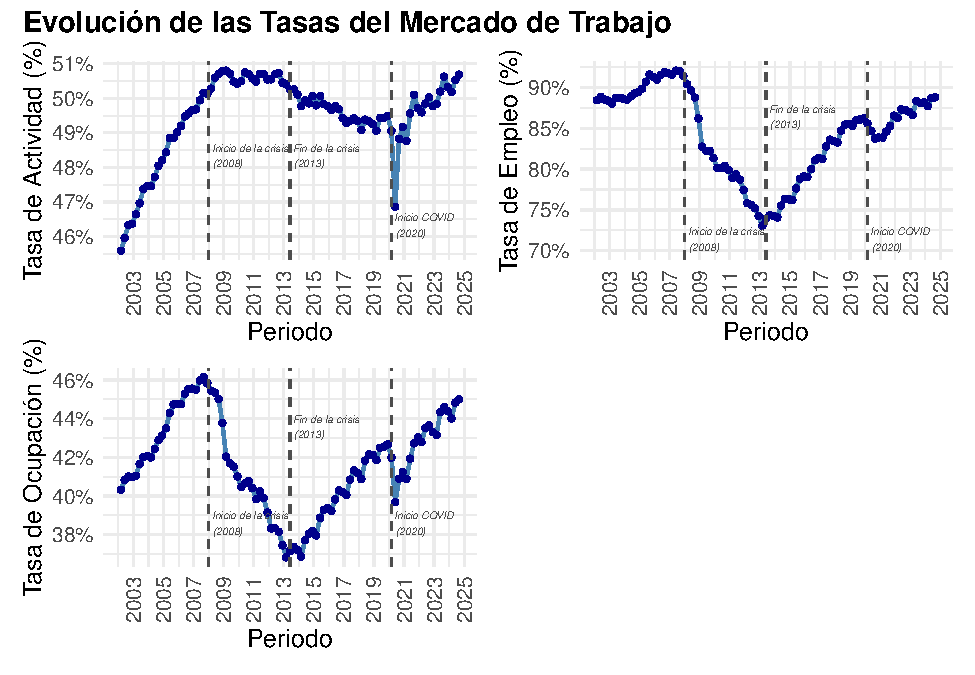
\includegraphics[width=1\linewidth]{ProyectoAED2024_files/figure-latex/unnamed-chunk-26-1} 

}

\caption{Evolución de la tasa de actividad en España}\label{fig:unnamed-chunk-26}
\end{figure}

La figura 1 muestra la evolución de tres indicadores clave del mercado
laboral en España: la tasa de actividad, la tasa de empleo y la tasa de
ocupación, desde 2002 hasta prácticamente la actualidad, reflejando
periodos de estabilidad y cambios abruptos relacionados con eventos
económicos y sociales. Entre 2002 y 2008, todas las tasas experimentan
un crecimiento sostenido, impulsado por la bonanza económica previa a la
crisis financiera global, con un auge en sectores como la construcción y
los servicios, y una incorporación activa de la población al mercado
laboral.

El inicio de la crisis en 2008 genera un comportamiento diferenciado:
mientras que la tasa de actividad se mantiene relativamente estable
hasta 2013, las tasas de empleo y ocupación muestran un descenso
significativo, reflejando el impacto directo de la destrucción de empleo
y la pérdida de capacidad de absorción del mercado laboral. Esto indica
que, aunque muchas personas siguieron buscando trabajo activamente
(evitando una caída en la actividad), el deterioro de las condiciones
laborales afectó severamente las oportunidades de empleo. La tasa de
empleo pasó de más del 90\% a por debajo del 75\% en 2013, o que es lo
mismo, un desempleo de más del 25\% en la población.

A partir de 2013, con los primeros signos de recuperación económica, la
tasa de actividad decrece levemente, posiblemente asociada a una menor
presión en el mercado laboral y una reducción del abandono escolar,
mientras que las tasas de empleo y ocupación comienzan una recuperación
progresiva. Este periodo refleja una estabilización del mercado laboral
con la recuperación de ciertos sectores clave.

El impacto de la pandemia de COVID-19 en 2020 es evidente en todas las
tasas, con caídas abruptas, especialmente en la tasa de ocupación,
debido al cierre temporal de actividades económicas y restricciones de
movilidad. Este impacto fue más pronunciado que el de la crisis
financiera. Desde 2021, se observa una recuperación acelerada en las
tres tasas, marcada por la reincorporación de trabajadores al mercado
laboral y el dinamismo de sectores como los servicios digitales, el
comercio y el turismo.

\begin{figure}[h]

{\centering 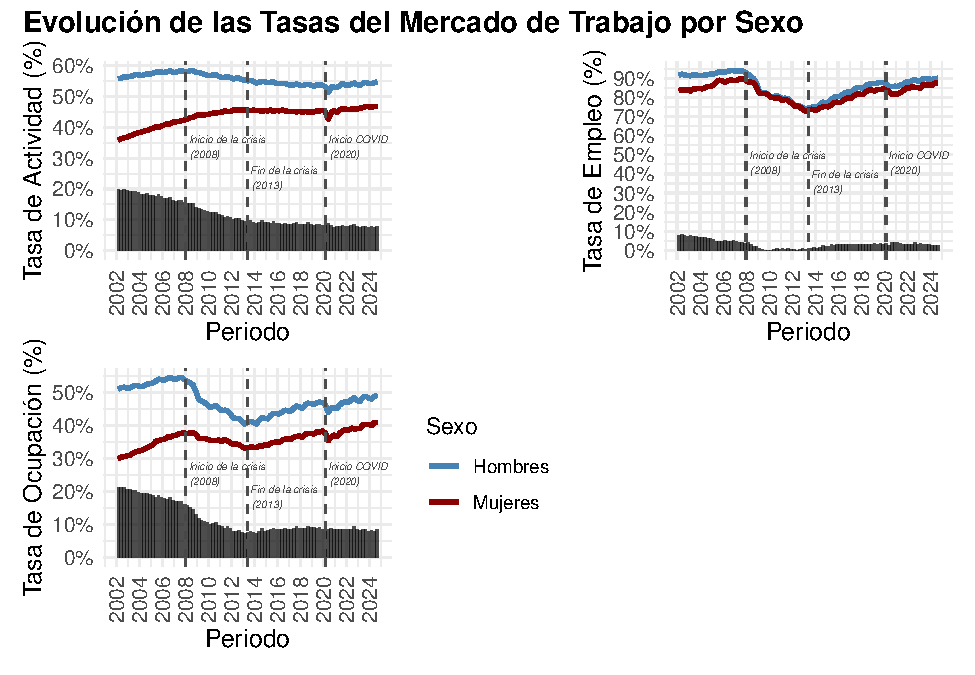
\includegraphics[width=1\linewidth]{ProyectoAED2024_files/figure-latex/unnamed-chunk-28-1} 

}

\caption{Evolución de la tasa de actividad en España}\label{fig:unnamed-chunk-28}
\end{figure}

La figura muestra la evolución de las tasas de actividad, empleo y
ocupación desglosadas por género, evidenciando patrones de desigualdad,
convergencia y algunas diferencias clave entre estos indicadores. La
tasa de actividad masculina, consistentemente más alta que la femenina,
experimenta un descenso gradual entre 2008 y 2020, probablemente
vinculado a los cambios estructurales tras la crisis financiera. En
contraste, la tasa de actividad femenina ha crecido de forma sostenida
desde 2002, impulsada por cambios sociales y legislativos, aunque este
crecimiento se ralentiza a partir de 2008. Este proceso ha reducido la
brecha de género de casi un 20\% en 2002 a cerca de un 8\% en años
recientes, como reflejan las barras grises que representan esta
diferencia.

En la tasa de empleo, sin embargo, las diferencias entre hombres y
mujeres son mucho más reducidas, lo que sugiere que la principal
disparidad radica en la población activa. Esto se explica porque la tasa
de empleo mide únicamente a las personas empleadas dentro de la
población activa, mientras que la tasa de ocupación considera a toda la
población en edad de trabajar. Por ello, las diferencias en la tasa de
ocupación entre hombres y mujeres son más marcadas, reflejando no solo
las desigualdades en el empleo, sino también las disparidades en la
incorporación al mercado laboral.

Durante la pandemia de COVID-19 en 2020, todas las tasas muestran un
descenso significativo, seguido de una recuperación que resalta la
resiliencia del mercado laboral. Este análisis pone en evidencia tanto
los avances hacia la igualdad de género en términos laborales como las
áreas donde persisten desigualdades estructurales, especialmente en la
población activa y su impacto en las tasas de ocupación.

\begin{figure}[h]

{\centering 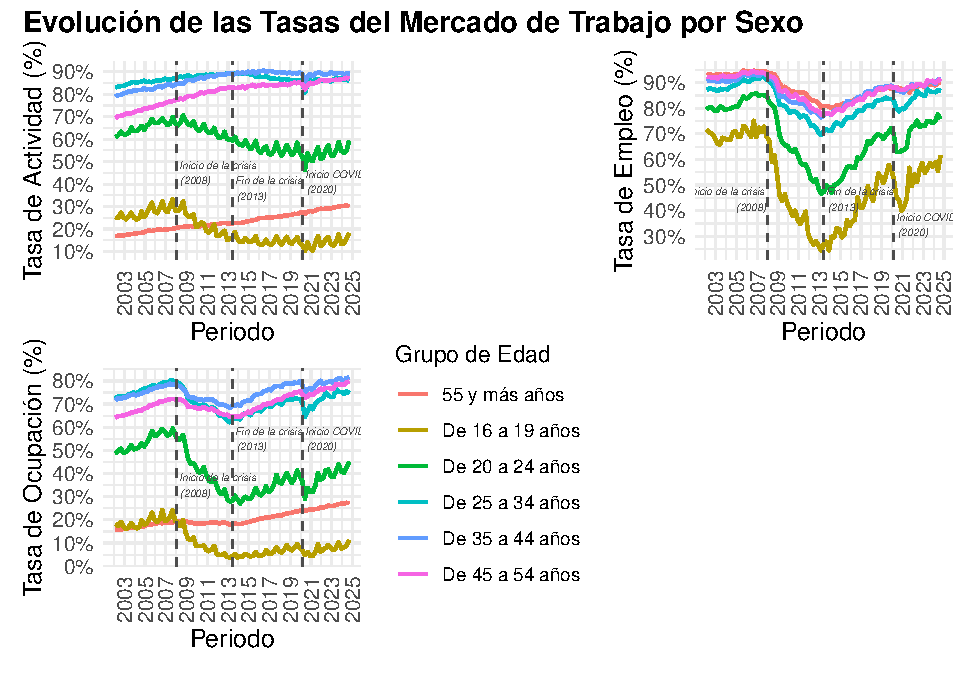
\includegraphics[width=1\linewidth]{ProyectoAED2024_files/figure-latex/unnamed-chunk-30-1} 

}

\caption{Evolución de la tasa de actividad en España}\label{fig:unnamed-chunk-30}
\end{figure}

Por último, desglosadando la población por grupos de edad, se puede
observar cómo cada segmento ha experimentado diferentes dinámicas en el
mercado laboral. Los grupos de mayor edad, como los de 35 a 44 años y 45
a 54 años, destacan por mantener tasas de actividad superiores al 80 \%,
significativamente más altas y estables a lo largo del tiempo,
reflejando su integración consolidada en el mercado laboral. En
contraste, los grupos más jóvenes, especialmente el de 16 a 19 años,
presentan tasas considerablemente más bajas, con una caída pronunciada
desde 2008. Por ejemplo, en 2013, la tasa de empleo de este grupo se
sitúa por debajo del 30 \%, lo que implica un desempleo superior al 70
\%. Este fenómeno puede atribuirse a que este grupo se encontraba
principalmente en el sector de la construcción, el cual sufrió más el
efecto de la recesión. Por otro lado, el aumento de la escolarización y
la prolongación de los estudios produjo la caída en su actividad.

Además, en los grupos jóvenes, como los de 16 a 19 años y 20 a 24 años,
se observa una marcada estacionalidad a lo largo del periodo,
probablemente vinculada a los meses de verano, cuando muchos estudiantes
se incorporan temporalmente al mercado laboral, especialmente en
sectores como la hostelería. Por su parte, en la tasa de actividad y
ocupación, el grupo de 55 y más años presenta niveles considerablemente
más bajos debido a la jubilación, ya que estos ciudadanos son
considerados población inactiva. Sin embargo, este fenómeno no se
refleja de la misma forma en la tasa de empleo, ya que este indicador se
calcula en función de la población activa, excluyendo a los inactivos
como los jubilados.

\subsubsection{Clusterización por Comunidades y Ciudades
Autónomas}\label{clusterizaciuxf3n-por-comunidades-y-ciudades-autuxf3nomas}

En este apartado del proyecto se va a proceder a realizar un clustering
de la tasa de empleo para las distintas Comunidades y Ciudades Autónomas
de España en los siguientes años: 2007, 2013 y 2023. El principal motivo
por el cual escogemos esta tasa se debe a que se mide como el porcentaje
de personas ocupadas respecto a la población activa, es decir, las que
se encuentran activamente en el mercado laboral.

Como método de clusterización se utilizará el k-means, que organiza los
datos en grupos basados en su similitud. Este algoritmo comienza
eligiendo un número de clusters (\texttt{k}) y seleccionando centroides
iniciales al azar. Cada punto se asigna al cluster cuyo centroide está
más cercano, y luego los centroides se recalculan como el promedio de
los puntos en cada grupo. Es un proceso que se repite hasta que los
centroides dejan de cambiar o se alcanza un límite de iteraciones. Al
finalizar, las comunidades quedan agrupadas en k clusters, representando
cada uno un conjunto de puntos con características similares.

Por otro lado, como método para la selección del hiperparámetro
\texttt{k} se opta por el método del codo. Este método Consiste en
graficar la suma de cuadrados dentro del cluster (WSS) frente a
distintos valores de \texttt{k}. El punto donde la disminución de WSS se
ralentiza significativamente, formando un ``codo'', indica el número
adecuado de clusters.

\begin{figure}[h]

{\centering 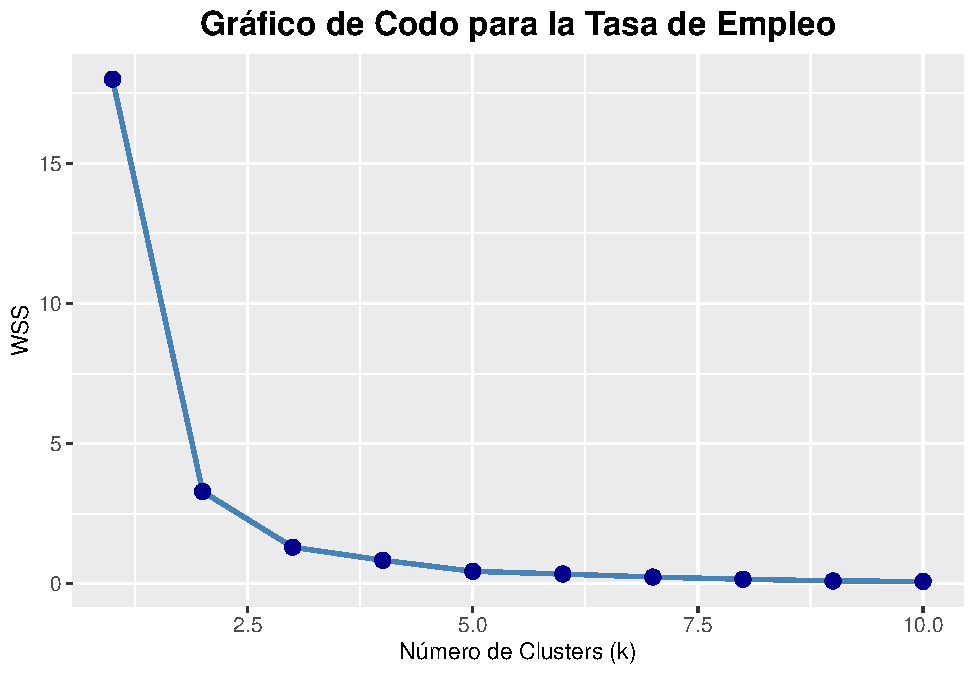
\includegraphics[width=0.6\linewidth]{ProyectoAED2024_files/figure-latex/unnamed-chunk-34-1} 

}

\caption{Evolución de la tasa de actividad en España}\label{fig:unnamed-chunk-34}
\end{figure}

Observando el gráfico anterior, se puede considerar que el número de
clusters a partir del cual la WSS se ralentiza es en \texttt{k=3}, pues
es en donde se forma el ``codo''.

Posteriormente, y como se ha mencionado al principio del apartado, vamos
a hacer un clustering con el objetivo de agrupar las CCAA según su tasa
de empleo en distintos periodos. Posteriormente los colores de los
clusters se representan en un mapa de España dividido por dichas
regiones para visualizar de forma clara y efectiva los patrones
espaciales.

La intención de esta medida es identificar patrones regionales y
analizar las diferencias en las dinámicas del mercado laboral a nivel
territorial. Este enfoque permite agrupar regiones con características
similares, facilitando la comparación interregional y destacando
aquellas con tasas de empleo altas, medias o bajas. Además, es útil para
detectar desigualdades laborales y sectoriales entre regiones
comprendendiendo cómo estas evolucionan a lo largo del tiempo.

\begin{figure}[h]

{\centering 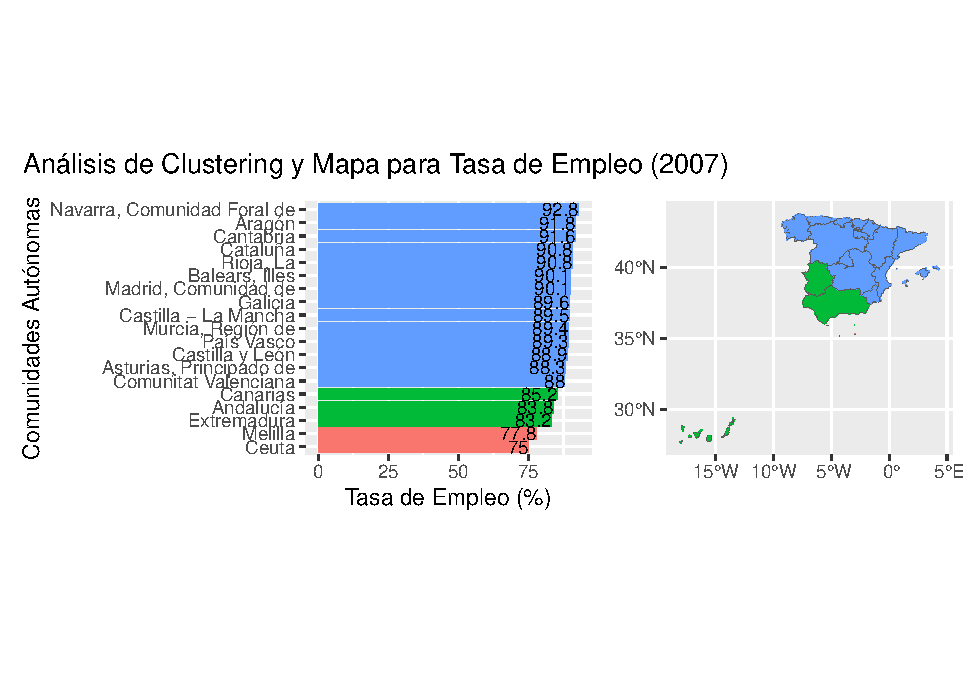
\includegraphics[width=1\linewidth]{ProyectoAED2024_files/figure-latex/unnamed-chunk-35-1} 

}

\caption{Evolución de la tasa de actividad en España}\label{fig:unnamed-chunk-35}
\end{figure}

La figura muestra el análisis de clustering y el mapa correspondiente a
la tasa de empleo de las comunidades autónomas en España en el año 2007,
justo antes del inicio de la crisis financiera. En el gráfico de barras,
se observa que comunidades como Navarra, Aragón, Cantabria y Cataluña
presentan las tasas de empleo más altas, superando el 90\%. Estas
regiones, representadas en azul en el mapa, se agrupan en un mismo
clúster, lo que sugiere un desempeño laboral favorable en estas áreas,
posiblemente asociado a economías diversificadas y mercados laborales
más sólidos tales como el tecnológico o el industrial.

Por otro lado, comunidades como Ceuta, Melilla, Extremadura y Andalucía
tienen las tasas de empleo más bajas, por debajo del 85\%, y se agrupan
en un clúster diferenciado, marcado en rojo en el mapa. Esto refleja un
mercado laboral más débil en estas regiones, históricamente
caracterizadas por mayores tasas de desempleo y una dependencia
económica de sectores menos dinámicos.

El clúster intermedio, representado en verde, incluye comunidades como
Galicia, Castilla-La Mancha y Murcia, con tasas de empleo moderadas,
entre el 85\% y el 90\%. Este grupo muestra un desempeño laboral
estable, aunque menos destacado en comparación con las regiones líderes.

En su conjunto, la figura permite identificar con claridad las
disparidades regionales en el mercado laboral español en 2007 desde el
sur hasta el norte del país, proporcionando una línea base para evaluar
cómo estas dinámicas se vieron afectadas por la crisis económica que
comenzaría poco después.

\begin{figure}[h]

{\centering 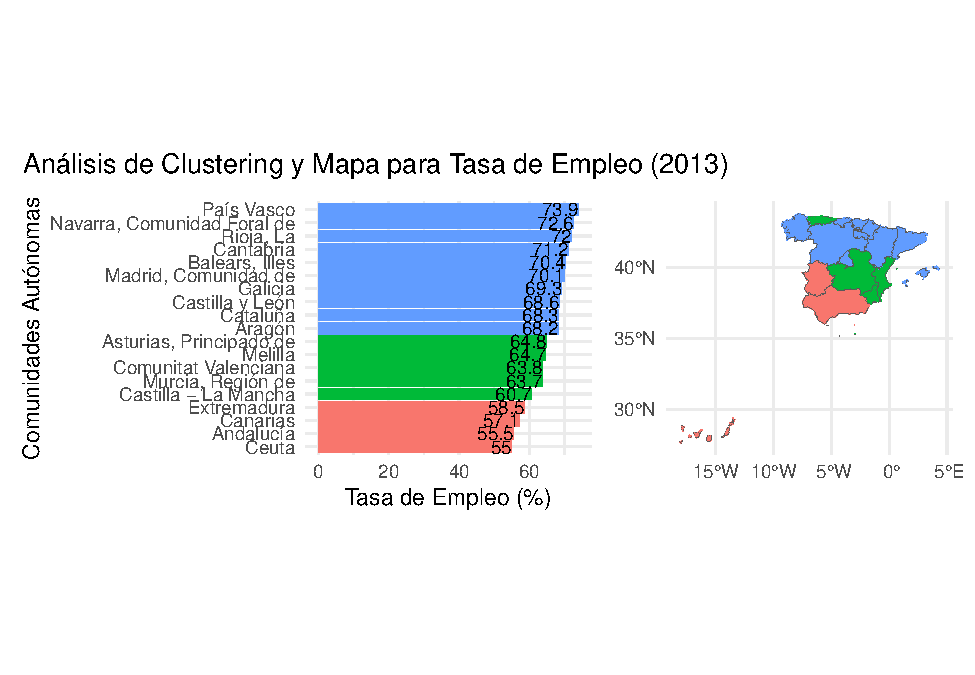
\includegraphics[width=1\linewidth]{ProyectoAED2024_files/figure-latex/unnamed-chunk-36-1} 

}

\caption{Evolución de la tasa de actividad en España}\label{fig:unnamed-chunk-36}
\end{figure}

Por otro lado, la figura muestra el análisis de clustering y el mapa en
2013, el momento más crítico de la crisis económica en España. En
comparación con 2007, se observa una disminución generalizada de las
tasas de empleo en todas las regiones, reflejando el impacto severo de
la crisis en el mercado laboral. Las comunidades con tasas de empleo más
altas, como País Vasco, La Rioja y Navarra, apenas superan el 70\%,
situándose muy por debajo de los niveles precrisis que superaban el
90\%. Estas regiones, representadas en azul en el mapa, se mantienen
como las de mejor desempeño relativo, aunque con una caída significativa
respecto a 2007.

Las comunidades con tasas más bajas, como Andalucía, Canarias y
Extremadura, presentan tasas de empleo inferiores al 60\%, destacando
Andalucía con un preocupante 55.5\%. Este grupo, representado en rojo en
el mapa, evidencia el fuerte deterioro del mercado laboral en regiones
tradicionalmente más vulnerables, donde la crisis intensificó los
problemas estructurales de empleo.

El clúster intermedio, en verde, agrupa comunidades como Galicia,
Castilla y León, y Cataluña, con tasas de empleo entre el 63\% y el
70\%. Este grupo muestra una reducción importante en comparación con los
niveles previos a la crisis, pero logra mantenerse en un rango moderado
frente a las regiones con peor desempeño.

En conjunto, la figura refleja cómo la crisis económica impactó de
manera desigual en el territorio español, exacerbando las disparidades
regionales en el empleo. Aunque las regiones líderes lograron mantener
una relativa ventaja, la caída generalizada evidencia la magnitud del
daño económico y social provocado por la crisis. Este análisis destaca
la importancia de entender las dinámicas regionales para diseñar
políticas efectivas de recuperación y fortalecimiento del mercado
laboral.

\begin{figure}[h]

{\centering 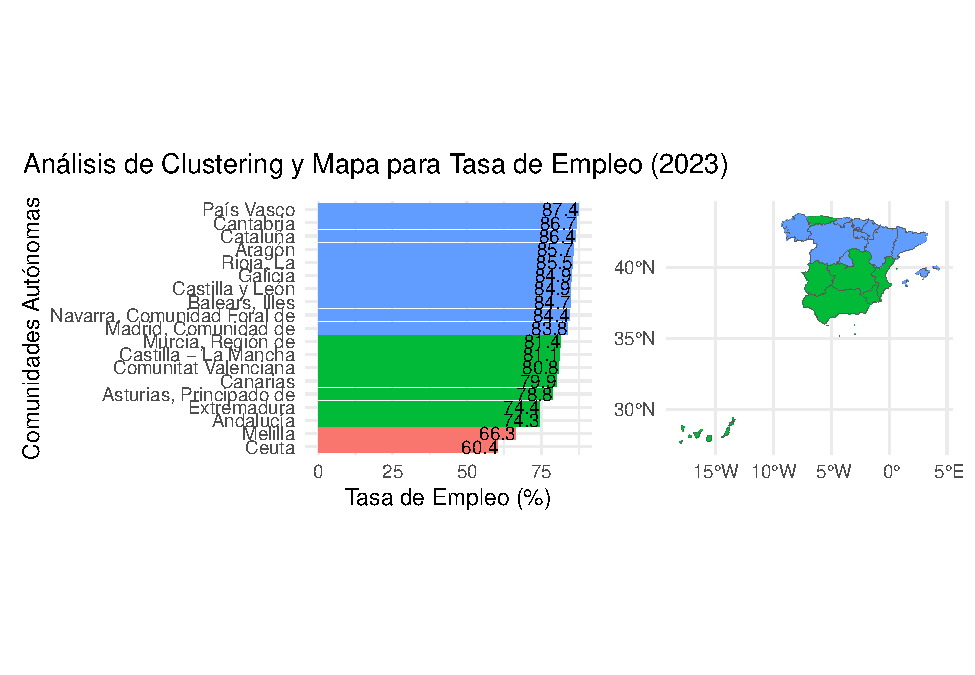
\includegraphics[width=1\linewidth]{ProyectoAED2024_files/figure-latex/unnamed-chunk-37-1} 

}

\caption{Evolución de la tasa de actividad en España}\label{fig:unnamed-chunk-37}
\end{figure}

Por último lugar, y relacionado con la actualidad, la figura de 2023
refleja una clara recuperación del mercado laboral tras los efectos de
la crisis económica de 2008-2013 y la pandemia de COVID-19. Comparado
con 2007, la tasa de empleo aún no alcanza los niveles previos a la
crisis, pero muestra una mejora significativa respecto a 2013, lo que
indica una tendencia hacia la estabilización y el fortalecimiento del
empleo en el país.

En 2023, las comunidades con mejor desempeño, representadas en azul,
poseen tasas de empleo que superan el 84\%. Aunque aún por debajo del
90\% que caracterizaba a las regiones líderes en 2007, estas comunidades
han logrado una recuperación considerable desde 2013, cuando sus tasas
apenas superaban el 70\%.

El grupo intermedio, representado en verde, posee unos valores de empleo
alrededor del 80\%. Este grupo muestra una notable mejora frente a los
niveles de 2013, cuando sus tasas se encontraban en torno al 65\%-70\%.
La recuperación en estas regiones evidencia un crecimiento sostenido que
les permite acercarse al desempeño de las regiones líderes.

Las comunidades con menor tasa de empleo, como Ceuta, Melilla, Andalucía
y Extremadura, representadas en rojo, registran tasas por debajo del
75\%. Aunque muestran avances significativos respecto a 2013, cuando sus
tasas eran inferiores al 60\%, estas regiones siguen siendo las más
afectadas por problemas estructurales en el mercado laboral. Andalucía,
por ejemplo, ha alcanzado una tasa del 74.3\%, un progreso importante
desde el 55.5\% en 2013, pero aún distante de las regiones con mejor
desempeño.

En conclusión, en comparación con 2007 el panorama de 2023 refleja un
mercado laboral más o menos parecido pero con más desempleo,
persistiendo también las disparidades regionales. Las comunidades más
vulnerables han avanzado considerablemente, pero no han cerrado la
brecha con las regiones líderes. Este análisis realizado con clustering
subraya la importancia de continuar impulsando políticas orientadas a
fortalecer el empleo en las regiones más rezagadas, fomentando la
cohesión territorial y reduciendo las desigualdades en el mercado
laboral español.

\subsection{Clasificación Nacional de Actividades Económicas
(CNAE-2009)}\label{clasificaciuxf3n-nacional-de-actividades-econuxf3micas-cnae-2009-1}

En primer lugar se analiza la distribución de peso de las ramas de
actividad en el total de la población empleada. Además, se busca
comparar la evolución y el cambio sufrido por la estructura laboral
española desde el primer trimestre de 2008 y el tercer trimestre de
2024. Para ello se generan treemaps para los periodos inicial (2008T1) y
final (2024T3) del análisis. Estos gráficos muestran cómo se distribuye
el empleo entre las diferentes ramas económicas según su peso relativo.

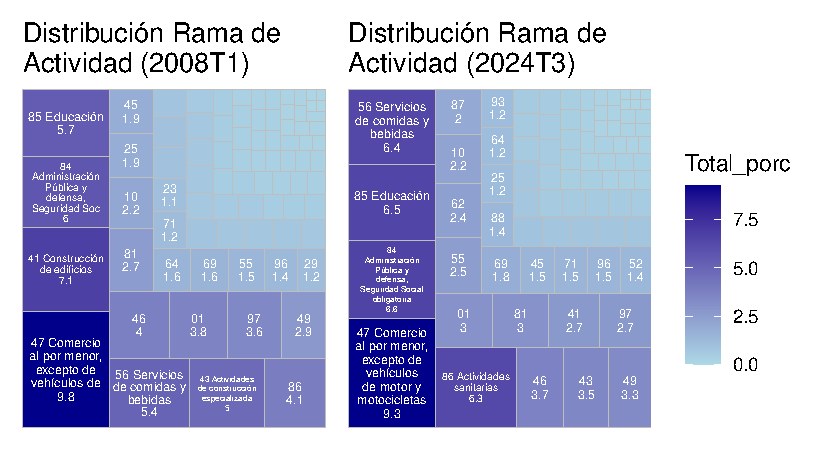
\includegraphics{ProyectoAED2024_files/figure-latex/unnamed-chunk-38-1.pdf}
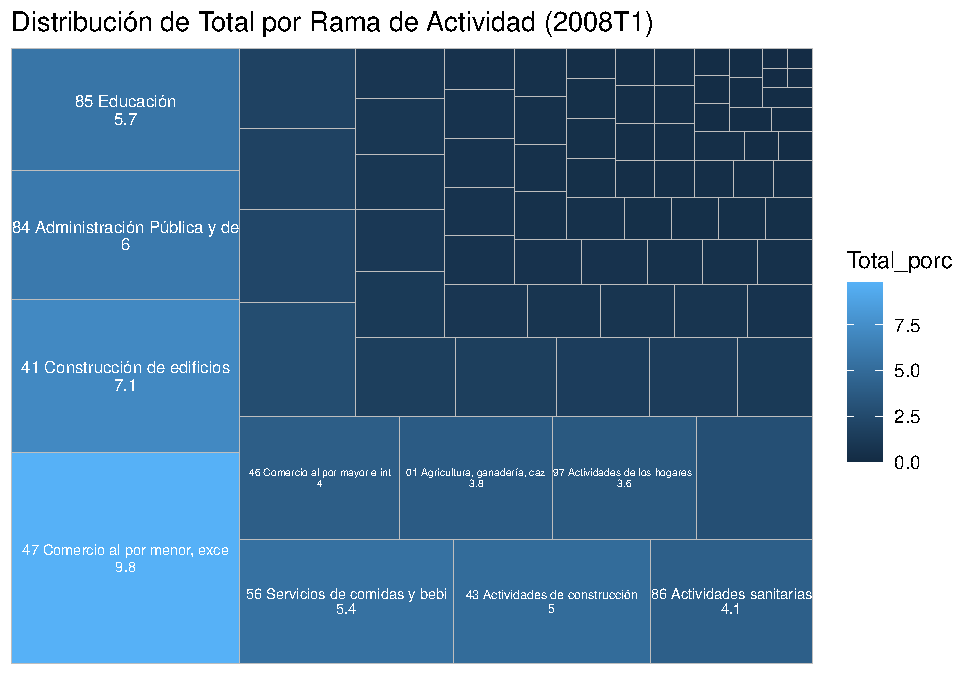
\includegraphics{ProyectoAED2024_files/figure-latex/unnamed-chunk-38-2.pdf}
Se observa cómo algunas ramas han ganado o perdido relevancia en
términos de empleo total a lo largo del tiempo. Por ejemplo, sectores
relacionados con la educación y la administración pública han aumentado
su proporción, mientras que ramas relacionadas con la construcción y la
industria han experimentado una marcada disminución.

Además de realizar un análisis comparativo de cómo se distribuye por
ramas de actividad la población trabajadora, se realiza un análisis
visual de la evolución del empleo en España de manera absoluta agrupando
por sexo, en conjunto con un análisis de la evolución de la diferencia
trimestral en el empleo. Para ello se han empleado gráficos de lineas.
Estos gráficos incluyen referencias visuales a eventos históricos
relevantes, como el fin de la crisis económica de 2013 y el inicio de la
pandemia en 2020.

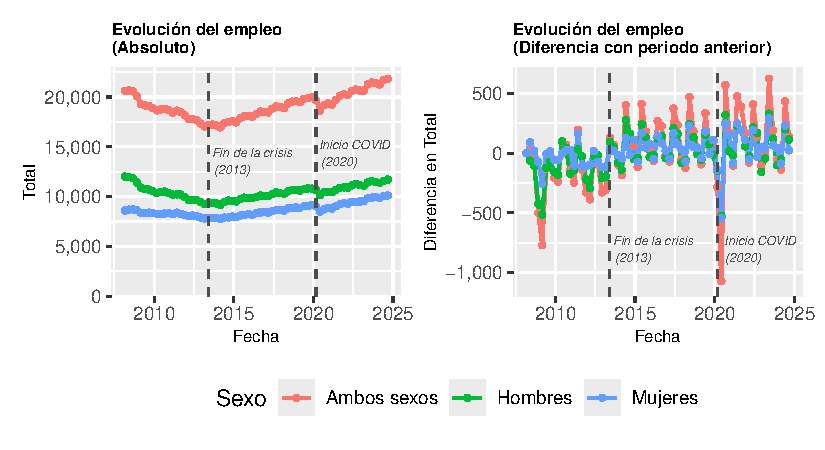
\includegraphics{ProyectoAED2024_files/figure-latex/unnamed-chunk-39-1.pdf}

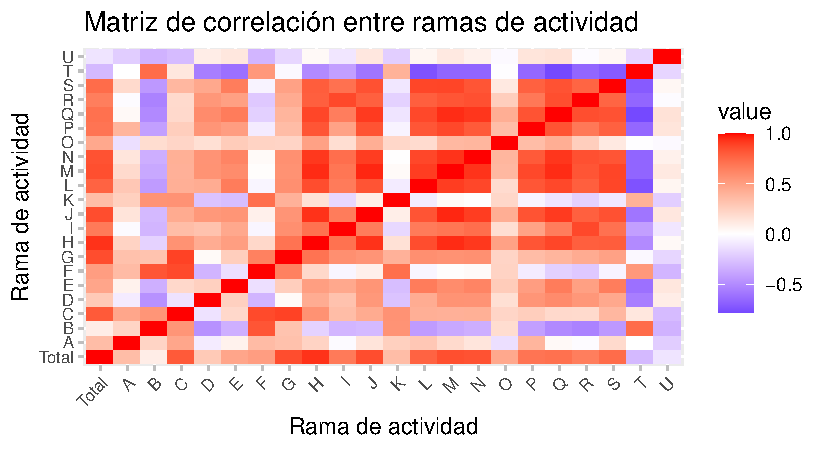
\includegraphics{ProyectoAED2024_files/figure-latex/unnamed-chunk-40-1.pdf}

Se destaca cómo el empleo masculino y femenino responden de manera
diferente a los shocks económicos. Por ejemplo, los hombres
experimentaron caídas más pronunciadas durante la crisis de 2008,
mientras que las mujeres mostraron una recuperación más gradual. Además,
se puede apreciar que la diferencia entre sexos se redujo en grán medida
durante la crisis de 2008, desde la cual la población masculina ha sido
incapaz de recuperar las cifras precrisis, mientras que las mujeres han
superado marcadamente dichos valores.

\subsubsection{Estudio de correlaciones entre Ramas de
Actividad}\label{estudio-de-correlaciones-entre-ramas-de-actividad}

A continuación, se realiza un estudio de las correlaciones lineales de
Pearson entre distintas ramas de actividad (en ambos sexos en conjunto).
Los datos de CNAE vienen dispuestos en dos órdenes de agrupación, unos
más generales, caracterizados por empezar por una letra en su nombre, y
otros más concretos, empezando por un número. Es por ello que se
realizan dos gráficas separadas que muestran la matriz de correlaciones
entre ramas.

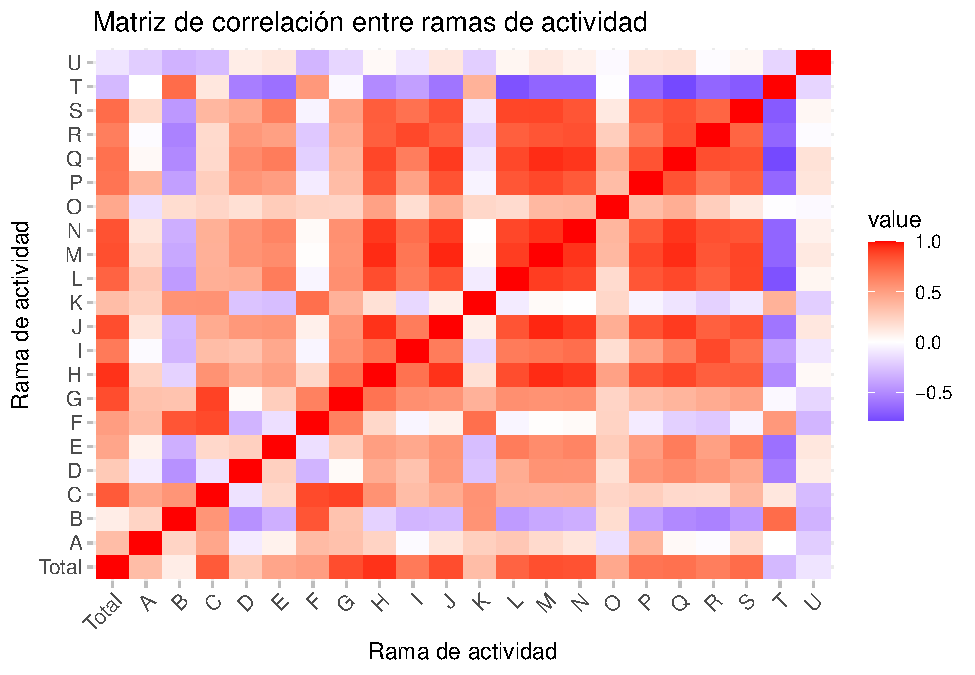
\includegraphics{ProyectoAED2024_files/figure-latex/unnamed-chunk-41-1.pdf}

Se observa que la mayoría de las ramas parecen estar correlacionadas
positivamente, salvo aquellos puestos relacionados con el personal
doméstico e industrias extractivas con una correlación negativa con la
mayoría de las ramas, así como aquellas relacionadas con la agricultura,
ganadería, construcción, actividades financieras entre otras que no
presentan una marcada correlación con el resto.

\subsubsection{Tendencias relativas a partir de datos
normalizados}\label{tendencias-relativas-a-partir-de-datos-normalizados}

En este punto, se busca estudiar las tendencias relativas, eliminando la
influencia de las diferencias inciales entre ramas. Para ello, primero
se normalizan los datos dividiendo por el número inicial de trabajadores
en cada rama, y a continuación se obtiene una métrica de distancia entre
dichos datos normalizados, obteniéndose como la media de las diferencias
absolutas de las cantidades normalizadas. A partir de estas distancias,
se proyectan en dos dimensiones utilizando MDS, lo que permite
visualizar las relaciones entre ramas en función de sus patrones de
empleo a lo largo del tiempo.

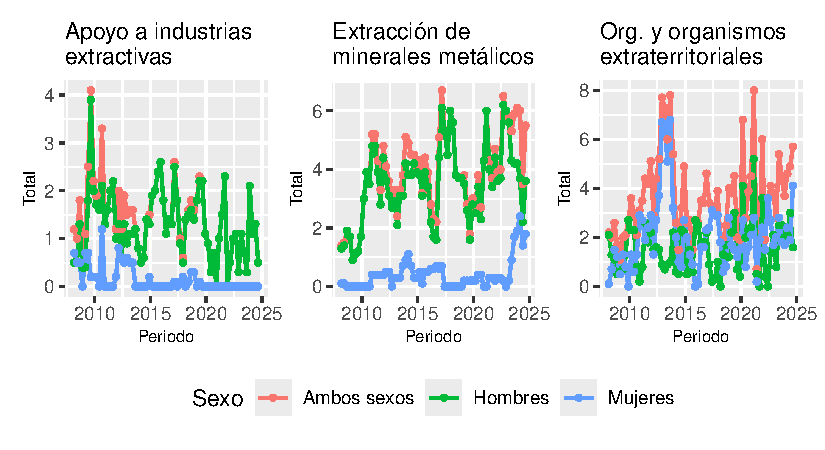
\includegraphics{ProyectoAED2024_files/figure-latex/unnamed-chunk-43-1.pdf}

Se forman agrupaciones naturales de ramas con patrones similares.
Además, se observan claramente algunos outliers, que puede ser de gran
interés analizarlos individualmente.

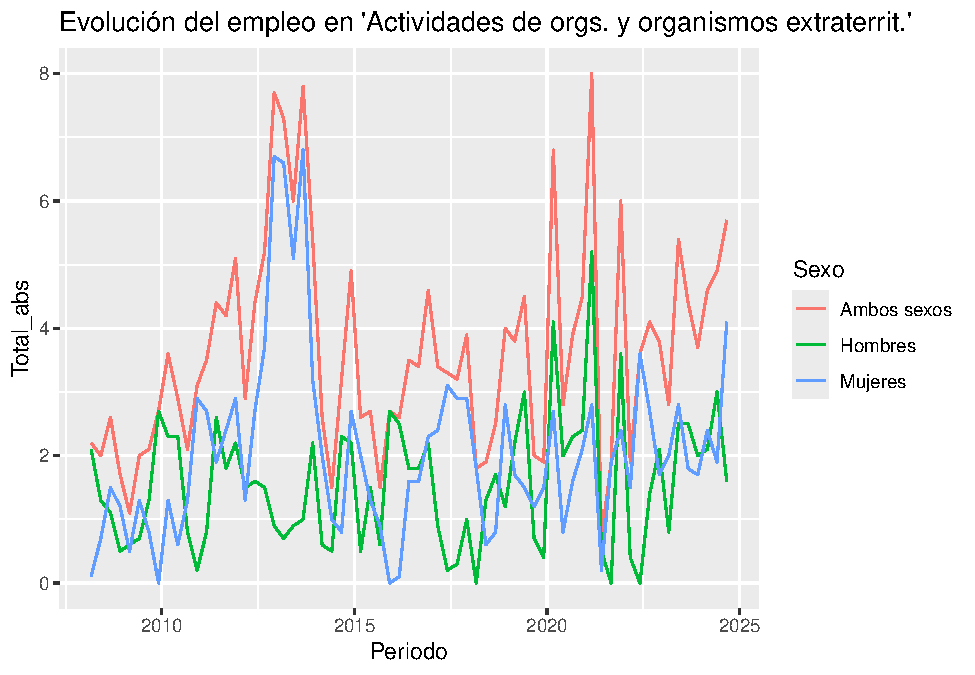
\includegraphics{ProyectoAED2024_files/figure-latex/unnamed-chunk-44-1.pdf}
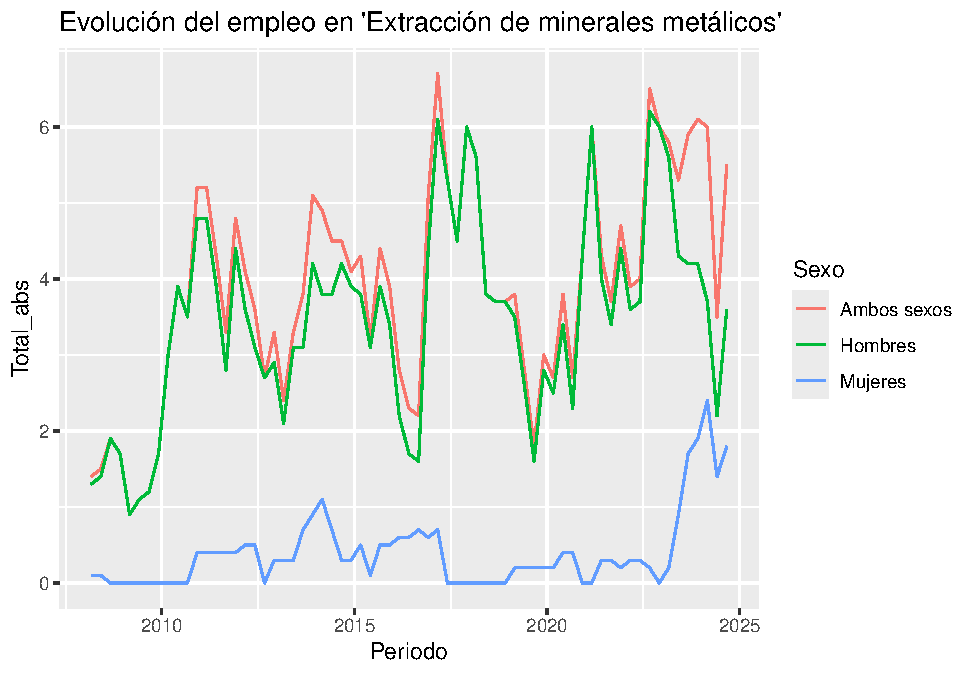
\includegraphics{ProyectoAED2024_files/figure-latex/unnamed-chunk-44-2.pdf}

Ramas como ``Extracción de minerales metálicos'' y ``Actividades de
organismos extraterritoriales'' se destacan por su comportamiento
atípico. Estas ramas tienen una dinámica de empleo inusual debido a su
naturaleza específica, tamaño reducido o dependencia de factores
externos como la demanda global. Observamos claramente que son datos con
mucho ruido y un gran incremento en los últimos años, y por lo tanto es
normal que nos apareciesen como outliers.

\subsubsection{Clusterización por Ramas de
Actividad}\label{clusterizaciuxf3n-por-ramas-de-actividad}

Tras observar la proyección tratamos de segmentar los datos en
agrupaciones naturales, es por ello que tratamos de hacer un clustering
que nos permita agrupar cuantitativamente aquellas ramas de actividad
que han tenido un comportamiento similar entre ellas (con los datos
normalizados). Para ello se opta en primer lugar por el algoritmo más
típico en clustering (k-means), y se analiza sus resultados para ver si
son satisfactorios. Además, como método para la selección del
hiperparámetro \texttt{k}, se opta por el método del codo. Sin embargo,
este resultado se analizará para saber si es adecuado, si sería
necesario alterar ligeramente el número de clusters obtenidos o si
directamente deberíamos escoger otro método.

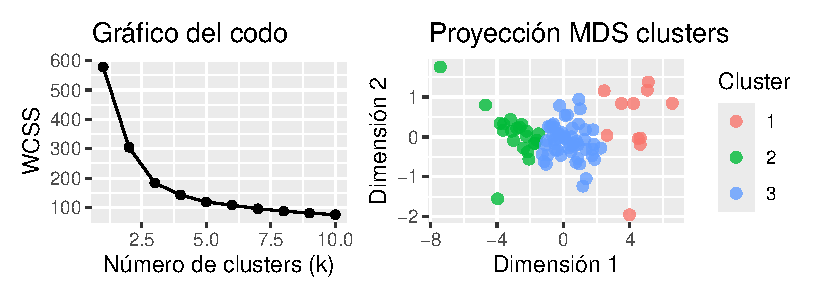
\includegraphics{ProyectoAED2024_files/figure-latex/unnamed-chunk-45-1.pdf}

A pesar que la gráfica del codo parece indicar que el mejor es
\texttt{k=4}, como se observa que al añadir el quinto lo que hace es
crear un cluster propio para los outliers, optamos por coger
\texttt{k=5}, pues esto puede ser beneficioso para eliminar el ruido de
estos sin la necesidad de eliminarlos de por si.

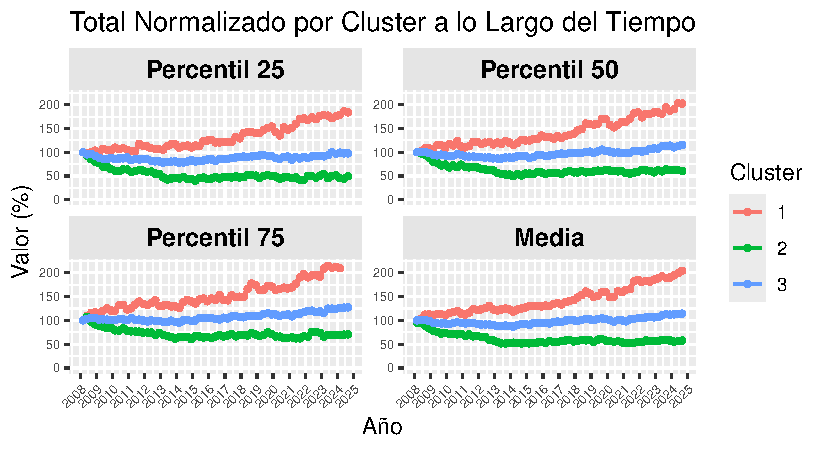
\includegraphics{ProyectoAED2024_files/figure-latex/unnamed-chunk-46-1.pdf}

Los resultados con k-means parecen positivos, por lo que por simplicidad
del modelo nos quedamos con esta elección. Pasamos a estudiar por
separado el comportamiento de cada cluster y trataremos de averiguar si
tienen una interpretación natural clara.

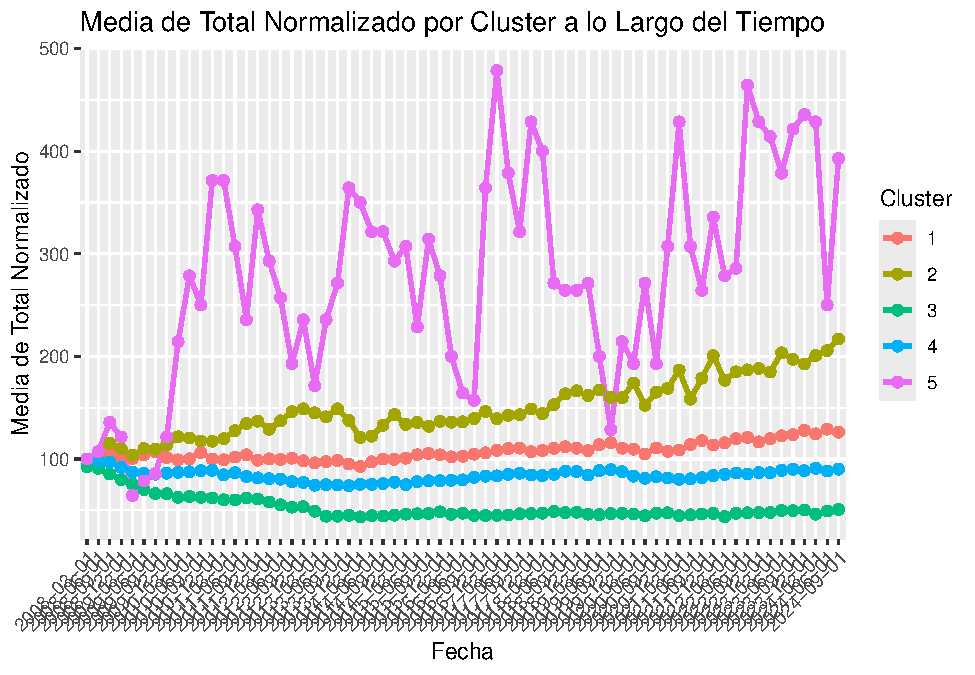
\includegraphics{ProyectoAED2024_files/figure-latex/unnamed-chunk-47-1.pdf}

\begin{Shaded}
\begin{Highlighting}[]
\NormalTok{data\_wide}\SpecialCharTok{$}\NormalTok{Cluster }\OtherTok{\textless{}{-}} \FunctionTok{as.factor}\NormalTok{(mds\_data}\SpecialCharTok{$}\NormalTok{Cluster)}

\NormalTok{data\_long }\OtherTok{\textless{}{-}}\NormalTok{ data\_wide }\SpecialCharTok{\%\textgreater{}\%}
  \FunctionTok{pivot\_longer}\NormalTok{(}\SpecialCharTok{{-}}\FunctionTok{c}\NormalTok{(Rama.de.actividad.CNAE}\FloatTok{.2009}\NormalTok{, Cluster), }\AttributeTok{names\_to =} \StringTok{"Periodo"}\NormalTok{, }\AttributeTok{values\_to =} \StringTok{"Total\_Normalizado"}\NormalTok{)}

\NormalTok{cuantiles\_por\_cluster }\OtherTok{\textless{}{-}}\NormalTok{ data\_long }\SpecialCharTok{\%\textgreater{}\%}
  \FunctionTok{group\_by}\NormalTok{(Cluster, Periodo) }\SpecialCharTok{\%\textgreater{}\%}
  \FunctionTok{summarise}\NormalTok{(}
    \AttributeTok{Cuantil\_25 =} \FunctionTok{quantile}\NormalTok{(Total\_Normalizado, }\FloatTok{0.25}\NormalTok{, }\AttributeTok{na.rm =} \ConstantTok{TRUE}\NormalTok{),}
    \AttributeTok{Cuantil\_50 =} \FunctionTok{quantile}\NormalTok{(Total\_Normalizado, }\FloatTok{0.50}\NormalTok{, }\AttributeTok{na.rm =} \ConstantTok{TRUE}\NormalTok{),}
    \AttributeTok{Cuantil\_75 =} \FunctionTok{quantile}\NormalTok{(Total\_Normalizado, }\FloatTok{0.75}\NormalTok{, }\AttributeTok{na.rm =} \ConstantTok{TRUE}\NormalTok{),}
    \AttributeTok{.groups =} \StringTok{\textquotesingle{}drop\textquotesingle{}}
\NormalTok{  ) }\SpecialCharTok{\%\textgreater{}\%}
  \FunctionTok{pivot\_longer}\NormalTok{(}\SpecialCharTok{{-}}\FunctionTok{c}\NormalTok{(Cluster, Periodo), }\AttributeTok{names\_to =} \StringTok{"Cuantil"}\NormalTok{, }\AttributeTok{values\_to =} \StringTok{"Valor"}\NormalTok{)}

\NormalTok{grafico\_cuantiles }\OtherTok{\textless{}{-}} \FunctionTok{ggplot}\NormalTok{(cuantiles\_por\_cluster, }\FunctionTok{aes}\NormalTok{(}\AttributeTok{x =}\NormalTok{ Periodo, }\AttributeTok{y =}\NormalTok{ Valor, }\AttributeTok{color =}\NormalTok{ Cluster, }\AttributeTok{group =} \FunctionTok{interaction}\NormalTok{(Cluster, Cuantil))) }\SpecialCharTok{+}
  \FunctionTok{geom\_line}\NormalTok{(}\AttributeTok{size =} \DecValTok{1}\NormalTok{) }\SpecialCharTok{+}
  \FunctionTok{geom\_point}\NormalTok{(}\AttributeTok{size =} \DecValTok{2}\NormalTok{) }\SpecialCharTok{+}
  \FunctionTok{facet\_wrap}\NormalTok{(}\SpecialCharTok{\textasciitilde{}}\NormalTok{ Cuantil, }\AttributeTok{nrow =} \DecValTok{3}\NormalTok{, }\AttributeTok{scales =} \StringTok{"free\_y"}\NormalTok{) }\SpecialCharTok{+} 
  \FunctionTok{labs}\NormalTok{(}\AttributeTok{title =} \StringTok{"Cuantiles de Total Normalizado por Cluster a lo Largo del Tiempo"}\NormalTok{,}
       \AttributeTok{x =} \StringTok{"Fecha"}\NormalTok{, }\AttributeTok{y =} \StringTok{"Valor"}\NormalTok{) }\SpecialCharTok{+}
  \FunctionTok{theme}\NormalTok{(}\AttributeTok{axis.text.x =} \FunctionTok{element\_text}\NormalTok{(}\AttributeTok{angle =} \DecValTok{45}\NormalTok{, }\AttributeTok{hjust =} \DecValTok{1}\NormalTok{)) }

\FunctionTok{print}\NormalTok{(grafico\_cuantiles)}
\end{Highlighting}
\end{Shaded}

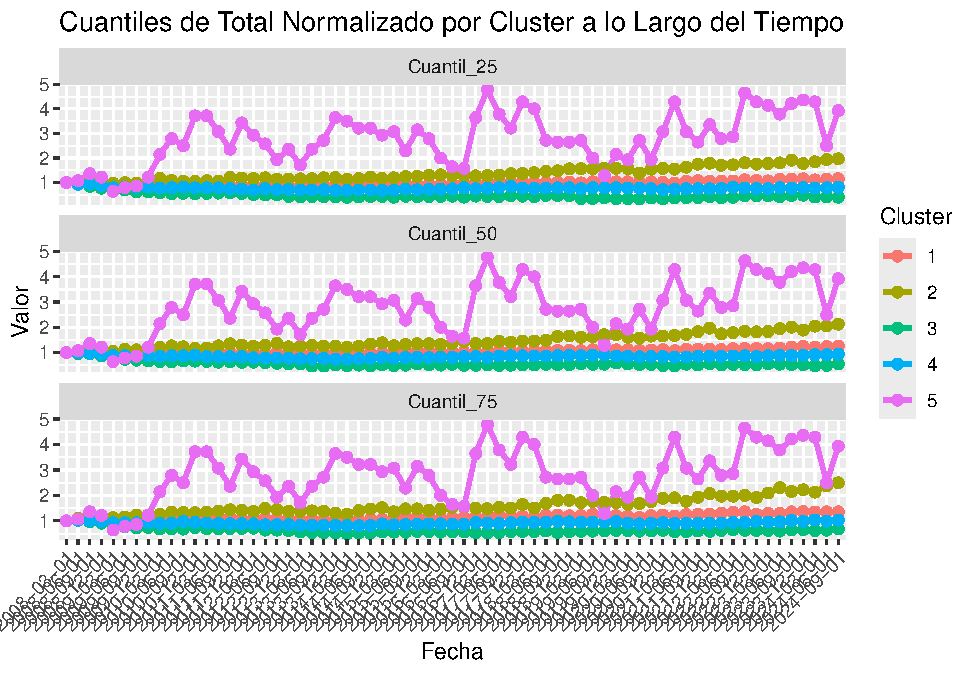
\includegraphics{ProyectoAED2024_files/figure-latex/unnamed-chunk-48-1.pdf}

\begin{Shaded}
\begin{Highlighting}[]
\NormalTok{lista\_ramas\_por\_cluster }\OtherTok{\textless{}{-}}\NormalTok{ data\_wide }\SpecialCharTok{\%\textgreater{}\%}
  \FunctionTok{group\_by}\NormalTok{(Cluster) }\SpecialCharTok{\%\textgreater{}\%}
  \FunctionTok{summarise}\NormalTok{(}\AttributeTok{Ramas =} \FunctionTok{list}\NormalTok{(}\FunctionTok{unique}\NormalTok{(Rama.de.actividad.CNAE}\FloatTok{.2009}\NormalTok{)), }\AttributeTok{.groups =} \StringTok{\textquotesingle{}drop\textquotesingle{}}\NormalTok{)}

\NormalTok{lista\_ramas }\OtherTok{\textless{}{-}} \FunctionTok{as.list}\NormalTok{(}\FunctionTok{setNames}\NormalTok{(lista\_ramas\_por\_cluster}\SpecialCharTok{$}\NormalTok{Ramas, lista\_ramas\_por\_cluster}\SpecialCharTok{$}\NormalTok{Cluster))}
\FunctionTok{print}\NormalTok{(}\FunctionTok{lapply}\NormalTok{(lista\_ramas, }\ControlFlowTok{function}\NormalTok{(x) }\FunctionTok{head}\NormalTok{(x, }\DecValTok{3}\NormalTok{)))}
\end{Highlighting}
\end{Shaded}

\begin{verbatim}
## $`1`
## [1] "09 Actividades de apoyo a las industrias extractivas"
## [2] "10 Industria de la alimentación"                     
## [3] "17 Industria del papel"                              
## 
## $`2`
## [1] "39 Actividades de descontaminación y otros servicios de gestión de residuos"     
## [2] "52 Almacenamiento y actividades anexas al transporte"                            
## [3] "62 Programación, consultoría y otras actividades relacionadas con la informática"
## 
## $`3`
## [1] "05 Extracción de antracita, hulla y lignito"
## [2] "08 Otras industrias extractivas"            
## [3] "12 Industria del tabaco"                    
## 
## $`4`
## [1] "01 Agricultura, ganadería, caza y servicios relacionados con las mismas"
## [2] "02 Silvicultura y explotación forestal"                                 
## [3] "03 Pesca y acuicultura"                                                 
## 
## $`5`
## [1] "07 Extracción de minerales metálicos"
\end{verbatim}

Analizando los cuantiles y medias de cada cluster, se observa que se
agrupan segun rendimiento durante los últimos 16 años, cosa a esperar
proviniendo de la métrica definida. Se observan que la mayoría de las
ramas de actividad se acumulan en los clústeres con la evolución
negativa, en los cuales ha habido un decrecimiento (cluster 5) o
estancamiento (cluster 4) de los trabajadores. Por otra parte el cluster
3 parece presentar ramas con ligeros resultados positivos, y el cluster
1 con marcados resultados positivos, aunque con menor número de ramas
que los anteriores. Por último, el cluster 2 se trata del cluster de
outliers.

%%%%%%%%%%%%%%%%%%%%%%%%%%%%%%%%%%%%%%%%%%

\vspace{6pt}

%%%%%%%%%%%%%%%%%%%%%%%%%%%%%%%%%%%%%%%%%%
%% optional

% Only for the journal Methods and Protocols:
% If you wish to submit a video article, please do so with any other supplementary material.
% \supplementary{The following supporting information can be downloaded at: \linksupplementary{s1}, Figure S1: title; Table S1: title; Video S1: title. A supporting video article is available at doi: link.}

%%%%%%%%%%%%%%%%%%%%%%%%%%%%%%%%%%%%%%%%%%







%%%%%%%%%%%%%%%%%%%%%%%%%%%%%%%%%%%%%%%%%%
%% Optional

%% Only for journal Encyclopedia


%%%%%%%%%%%%%%%%%%%%%%%%%%%%%%%%%%%%%%%%%%
%% Optional
%%%%%%%%%%%%%%%%%%%%%%%%%%%%%%%%%%%%%%%%%%
\begin{adjustwidth}{-\extralength}{0cm}

%\printendnotes[custom] % Un-comment to print a list of endnotes


\reftitle{References}
\bibliography{mybibfile.bib}

% If authors have biography, please use the format below
%\section*{Short Biography of Authors}
%\bio
%{\raisebox{-0.35cm}{\includegraphics[width=3.5cm,height=5.3cm,clip,keepaspectratio]{Definitions/author1.pdf}}}
%{\textbf{Firstname Lastname} Biography of first author}
%
%\bio
%{\raisebox{-0.35cm}{\includegraphics[width=3.5cm,height=5.3cm,clip,keepaspectratio]{Definitions/author2.jpg}}}
%{\textbf{Firstname Lastname} Biography of second author}

%%%%%%%%%%%%%%%%%%%%%%%%%%%%%%%%%%%%%%%%%%
%% for journal Sci
%\reviewreports{\\
%Reviewer 1 comments and authors’ response\\
%Reviewer 2 comments and authors’ response\\
%Reviewer 3 comments and authors’ response
%}
%%%%%%%%%%%%%%%%%%%%%%%%%%%%%%%%%%%%%%%%%%
\PublishersNote{}
\end{adjustwidth}


\end{document}
